\pdfoutput=1
%% bare_conf.tex
%% V1.4b
%% 2015/08/26
%% by Michael Shell
%% See:
%% http://www.michaelshell.org/
%% for current contact information.
%%
%% This is a skeleton file demonstrating the use of IEEEtran.cls
%% (requires IEEEtran.cls version 1.8b or later) with an IEEE
%% conference paper.
%%
%% Support sites:
%% http://www.michaelshell.org/tex/ieeetran/
%% http://www.ctan.org/pkg/ieeetran
%% and
%% http://www.ieee.org/

%%*************************************************************************
%% Legal Notice:
%% This code is offered as-is without any warranty either expressed or
%% implied; without even the implied warranty of MERCHANTABILITY or
%% FITNESS FOR A PARTICULAR PURPOSE! 
%% User assumes all risk.
%% In no event shall the IEEE or any contributor to this code be liable for
%% any damages or losses, including, but not limited to, incidental,
%% consequential, or any other damages, resulting from the use or misuse
%% of any information contained here.
%%
%% All comments are the opinions of their respective authors and are not
%% necessarily endorsed by the IEEE.
%%
%% This work is distributed under the LaTeX Project Public License (LPPL)
%% ( http://www.latex-project.org/ ) version 1.3, and may be freely used,
%% distributed and modified. A copy of the LPPL, version 1.3, is included
%% in the base LaTeX documentation of all distributions of LaTeX released
%% 2003/12/01 or later.
%% Retain all contribution notices and credits.
%% ** Modified files should be clearly indicated as such, including  **
%% ** renaming them and changing author support contact information. **
%%*************************************************************************


% *** Authors should verify (and, if needed, correct) their LaTeX system  ***
% *** with the testflow diagnostic prior to trusting their LaTeX platform ***
% *** with production work. The IEEE's font choices and paper sizes can   ***
% *** trigger bugs that do not appear when using other class files.       ***
% The testflow support page is at:
% http://www.michaelshell.org/tex/testflow/



\documentclass[conference]{IEEEtran}
% Some Computer Society conferences also require the compsoc mode option,
% but others use the standard conference format.
%
% If IEEEtran.cls has not been installed into the LaTeX system files,
% manually specify the path to it like:
% \documentclass[conference]{../sty/IEEEtran}





% Some very useful LaTeX packages include:
% (uncomment the ones you want to load)


% *** MISC UTILITY PACKAGES ***
%
%\usepackage{ifpdf}
% Heiko Oberdiek's ifpdf.sty is very useful if you need conditional
% compilation based on whether the output is pdf or dvi.
% usage:
% \ifpdf
%   % pdf code
% \else
%   % dvi code
% \fi
% The latest version of ifpdf.sty can be obtained from:
% http://www.ctan.org/pkg/ifpdf
% Also, note that IEEEtran.cls V1.7 and later provides a builtin
% \ifCLASSINFOpdf conditional that works the same way.
% When switching from latex to pdflatex and vice-versa, the compiler may
% have to be run twice to clear warning/error messages.



\usepackage[hidelinks]{hyperref}


% *** CITATION PACKAGES ***
%
\usepackage{cite}
% cite.sty was written by Donald Arseneau
% V1.6 and later of IEEEtran pre-defines the format of the cite.sty package
% \cite{} output to follow that of the IEEE. Loading the cite package will
% result in citation numbers being automatically sorted and properly
% "compressed/ranged". e.g., [1], [9], [2], [7], [5], [6] without using
% cite.sty will become [1], [2], [5]--[7], [9] using cite.sty. cite.sty's
% \cite will automatically add leading space, if needed. Use cite.sty's
% noadjust option (cite.sty V3.8 and later) if you want to turn this off
% such as if a citation ever needs to be enclosed in parenthesis.
% cite.sty is already installed on most LaTeX systems. Be sure and use
% version 5.0 (2009-03-20) and later if using hyperref.sty.
% The latest version can be obtained at:
% http://www.ctan.org/pkg/cite
% The documentation is contained in the cite.sty file itself.






% *** GRAPHICS RELATED PACKAGES ***
%
\ifCLASSINFOpdf
   \usepackage[pdftex]{graphicx}	
  % declare the path(s) where your graphic files are
  % \graphicspath{{../pdf/}{../jpeg/}}
  % and their extensions so you won't have to specify these with
  % every instance of \includegraphics
  % \DeclareGraphicsExtensions{.pdf,.jpeg,.png}
\else
  % or other class option (dvipsone, dvipdf, if not using dvips). graphicx
  % will default to the driver specified in the system graphics.cfg if no
  % driver is specified.
   \usepackage[dvips]{graphicx}
  % declare the path(s) where your graphic files are
  % \graphicspath{{../eps/}}
  % and their extensions so you won't have to specify these with
  % every instance of \includegraphics
  % \DeclareGraphicsExtensions{.eps}
\fi

% graphicx was written by David Carlisle and Sebastian Rahtz. It is
% required if you want graphics, photos, etc. graphicx.sty is already
% installed on most LaTeX systems. The latest version and documentation
% can be obtained at: 
% http://www.ctan.org/pkg/graphicx
% Another good source of documentation is "Using Imported Graphics in
% LaTeX2e" by Keith Reckdahl which can be found at:
% http://www.ctan.org/pkg/epslatex
%
% latex, and pdflatex in dvi mode, support graphics in encapsulated
% postscript (.eps) format. pdflatex in pdf mode supports graphics
% in .pdf, .jpeg, .png and .mps (metapost) formats. Users should ensure
% that all non-photo figures use a vector format (.eps, .pdf, .mps) and
% not a bitmapped formats (.jpeg, .png). The IEEE frowns on bitmapped formats
% which can result in "jaggedy"/blurry rendering of lines and letters as
% well as large increases in file sizes.
%
% You can find documentation about the pdfTeX application at:
% http://www.tug.org/applications/pdftex





% *** MATH PACKAGES ***
%
\usepackage{amsmath}
% A popular package from the American Mathematical Society that provides
% many useful and powerful commands for dealing with mathematics.
%
% Note that the amsmath package sets \interdisplaylinepenalty to 10000
% thus preventing page breaks from occurring within multiline equations. Use:
\interdisplaylinepenalty=2500
% after loading amsmath to restore such page breaks as IEEEtran.cls normally
% does. amsmath.sty is already installed on most LaTeX systems. The latest
% version and documentation can be obtained at:
% http://www.ctan.org/pkg/amsmath





% *** SPECIALIZED LIST PACKAGES ***
%
\usepackage{algorithmic}
% algorithmic.sty was written by Peter Williams and Rogerio Brito.
% This package provides an algorithmic environment fo describing algorithms.
% You can use the algorithmic environment in-text or within a figure
% environment to provide for a floating algorithm. Do NOT use the algorithm
% floating environment provided by algorithm.sty (by the same authors) or
% algorithm2e.sty (by Christophe Fiorio) as the IEEE does not use dedicated
% algorithm float types and packages that provide these will not provide
% correct IEEE style captions. The latest version and documentation of
% algorithmic.sty can be obtained at:
% http://www.ctan.org/pkg/algorithms
% Also of interest may be the (relatively newer and more customizable)
% algorithmicx.sty package by Szasz Janos:
% http://www.ctan.org/pkg/algorithmicx




% *** ALIGNMENT PACKAGES ***
%
\usepackage{array}
% Frank Mittelbach's and David Carlisle's array.sty patches and improves
% the standard LaTeX2e array and tabular environments to provide better
% appearance and additional user controls. As the default LaTeX2e table
% generation code is lacking to the point of almost being broken with
% respect to the quality of the end results, all users are strongly
% advised to use an enhanced (at the very least that provided by array.sty)
% set of table tools. array.sty is already installed on most systems. The
% latest version and documentation can be obtained at:
% http://www.ctan.org/pkg/array


% IEEEtran contains the IEEEeqnarray family of commands that can be used to
% generate multiline equations as well as matrices, tables, etc., of high
% quality.




% *** SUBFIGURE PACKAGES ***
\ifCLASSOPTIONcompsoc
  \usepackage[caption=false,font=normalsize,labelfont=sf,textfont=sf]{subfig}
\else
  \usepackage[caption=false,font=footnotesize]{subfig}
\fi
% subfig.sty, written by Steven Douglas Cochran, is the modern replacement
% for subfigure.sty, the latter of which is no longer maintained and is
% incompatible with some LaTeX packages including fixltx2e. However,
% subfig.sty requires and automatically loads Axel Sommerfeldt's caption.sty
% which will override IEEEtran.cls' handling of captions and this will result
% in non-IEEE style figure/table captions. To prevent this problem, be sure
% and invoke subfig.sty's "caption=false" package option (available since
% subfig.sty version 1.3, 2005/06/28) as this is will preserve IEEEtran.cls
% handling of captions.
% Note that the Computer Society format requires a larger sans serif font
% than the serif footnote size font used in traditional IEEE formatting
% and thus the need to invoke different subfig.sty package options depending
% on whether compsoc mode has been enabled.
%
% The latest version and documentation of subfig.sty can be obtained at:
% http://www.ctan.org/pkg/subfig




% *** FLOAT PACKAGES ***
%
%\usepackage{fixltx2e}
% fixltx2e, the successor to the earlier fix2col.sty, was written by
% Frank Mittelbach and David Carlisle. This package corrects a few problems
% in the LaTeX2e kernel, the most notable of which is that in current
% LaTeX2e releases, the ordering of single and double column floats is not
% guaranteed to be preserved. Thus, an unpatched LaTeX2e can allow a
% single column figure to be placed prior to an earlier double column
% figure.
% Be aware that LaTeX2e kernels dated 2015 and later have fixltx2e.sty's
% corrections already built into the system in which case a warning will
% be issued if an attempt is made to load fixltx2e.sty as it is no longer
% needed.
% The latest version and documentation can be found at:
% http://www.ctan.org/pkg/fixltx2e


%\usepackage{stfloats}
% stfloats.sty was written by Sigitas Tolusis. This package gives LaTeX2e
% the ability to do double column floats at the bottom of the page as well
% as the top. (e.g., "\begin{figure*}[!b]" is not normally possible in
% LaTeX2e). It also provides a command:
%\fnbelowfloat
% to enable the placement of footnotes below bottom floats (the standard
% LaTeX2e kernel puts them above bottom floats). This is an invasive package
% which rewrites many portions of the LaTeX2e float routines. It may not work
% with other packages that modify the LaTeX2e float routines. The latest
% version and documentation can be obtained at:
% http://www.ctan.org/pkg/stfloats
% Do not use the stfloats baselinefloat ability as the IEEE does not allow
% \baselineskip to stretch. Authors submitting work to the IEEE should note
% that the IEEE rarely uses double column equations and that authors should try
% to avoid such use. Do not be tempted to use the cuted.sty or midfloat.sty
% packages (also by Sigitas Tolusis) as the IEEE does not format its papers in
% such ways.
% Do not attempt to use stfloats with fixltx2e as they are incompatible.
% Instead, use Morten Hogholm'a dblfloatfix which combines the features
% of both fixltx2e and stfloats:
%
\usepackage{dblfloatfix}
% The latest version can be found at:
% http://www.ctan.org/pkg/dblfloatfix




% *** PDF, URL AND HYPERLINK PACKAGES ***
%
\usepackage{url}
% url.sty was written by Donald Arseneau. It provides better support for
% handling and breaking URLs. url.sty is already installed on most LaTeX
% systems. The latest version and documentation can be obtained at:
% http://www.ctan.org/pkg/url
% Basically, \url{my_url_here}.




% *** Do not adjust lengths that control margins, column widths, etc. ***
% *** Do not use packages that alter fonts (such as pslatex).         ***
% There should be no need to do such things with IEEEtran.cls V1.6 and later.
% (Unless specifically asked to do so by the journal or conference you plan
% to submit to, of course. )

%\usepackage{flushend}
\usepackage{mathabx}
\usepackage{booktabs}
\usepackage{multirow}
\usepackage{color}
\usepackage{bm}
\usepackage{xcolor}
\usepackage{pgfplots}
%\pgfplotsset{width=2in,compat=1.9}
%\usepackage{forest}
%\usetikzlibrary{arrows.meta, shapes.geometric, calc, shadows}
%\usepgfplotslibrary{external}
%\tikzexternalize


% correct bad hyphenation here
\hyphenation{op-tical net-works semi-conduc-tor}
\graphicspath{ {images/} }
\newtheorem{definition}{Definition}[section]
\newtheorem{principle}{Principle}

\makeatletter
\newcommand\xleftrightarrow[2][]{%
  \ext@arrow 9999{\longleftrightarrowfill@}{#1}{#2}}
\newcommand\longleftrightarrowfill@{%
  \arrowfill@\leftarrow\relbar\rightarrow}
\makeatother


\begin{document}
%
% paper title
% Titles are generally capitalized except for words such as a, an, and, as,
% at, but, by, for, in, nor, of, on, or, the, to and up, which are usually
% not capitalized unless they are the first or last word of the title.
% Linebreaks \\ can be used within to get better formatting as desired.
% Do not put math or special symbols in the title.
\title{Predicting Anchor Links between Heterogeneous Social Networks}


% author names and affiliations
% use a multiple column layout for up to three different
% affiliations
\author{
\IEEEauthorblockN{Sina Sajadmanesh}
\IEEEauthorblockA{Department of Computer Eng.\\
Sharif University of Technology\\
Email: sajadmanesh@ce.sharif.edu}
\and
\IEEEauthorblockN{Hamid R. Rabiee}
\IEEEauthorblockA{Department of Computer Eng.\\
Sharif University of Technology\\
Email: rabiee@sharif.edu}
\and
\IEEEauthorblockN{Ali Khodadadi}
\IEEEauthorblockA{Department of Computer Eng.\\
Sharif University of Technology\\
Email: khodadadi@ce.sharif.edu}
}

% conference papers do not typically use \thanks and this command
% is locked out in conference mode. If really needed, such as for
% the acknowledgment of grants, issue a \IEEEoverridecommandlockouts
% after \documentclass

% for over three affiliations, or if they all won't fit within the width
% of the page, use this alternative format:
% 
%\author{\IEEEauthorblockN{Michael Shell\IEEEauthorrefmark{1},
%Homer Simpson\IEEEauthorrefmark{2},
%James Kirk\IEEEauthorrefmark{3}, 
%Montgomery Scott\IEEEauthorrefmark{3} and
%Eldon Tyrell\IEEEauthorrefmark{4}}
%\IEEEauthorblockA{\IEEEauthorrefmark{1}School of Electrical and Computer Engineering\\
%Georgia Institute of Technology,
%Atlanta, Georgia 30332--0250\\ Email: see http://www.michaelshell.org/contact.html}
%\IEEEauthorblockA{\IEEEauthorrefmark{2}Twentieth Century Fox, Springfield, USA\\
%Email: homer@thesimpsons.com}
%\IEEEauthorblockA{\IEEEauthorrefmark{3}Starfleet Academy, San Francisco, California 96678-2391\\
%Telephone: (800) 555--1212, Fax: (888) 555--1212}
%\IEEEauthorblockA{\IEEEauthorrefmark{4}Tyrell Inc., 123 Replicant Street, Los Angeles, California 90210--4321}}




% use for special paper notices
%\IEEEspecialpapernotice{(Invited Paper)}




% make the title area
\maketitle

% As a general rule, do not put math, special symbols or citations
% in the abstract
\begin{abstract}
People usually get involved in multiple social networks to enjoy new services or to fulfill their needs. 
Many new social networks try to attract users of other existing networks to increase the number of their users. Once a user (called source user) of a social network (called source network) joins a new social network (called target network), a new inter-network link (called anchor link) is formed between the source and target networks. In this paper, we concentrated on predicting the formation of such anchor links between heterogeneous social networks. Unlike conventional link prediction problems in which the formation of a link between two existing users within a single network is predicted, in anchor link prediction, the target user is missing and will be added to the target network once the anchor link is created. To solve this problem, we use meta-paths as a powerful tool for utilizing heterogeneous information in both the source and target networks. To this end, we propose an effective general meta-path-based approach called \textit{Connector and Recursive Meta-Paths} (CRMP). By using those two different categories of meta-paths, we model different aspects of social factors that may affect a source user to join the target network, resulting in the formation of a new anchor link. Extensive experiments on real-world heterogeneous social networks demonstrate the effectiveness of the proposed method against the recent methods.

\end{abstract}

% no keywords




% For peer review papers, you can put extra information on the cover
% page as needed:
% \ifCLASSOPTIONpeerreview
% \begin{center} \bfseries EDICS Category: 3-BBND \end{center}
% \fi
%
% For peerreview papers, this IEEEtran command inserts a page break and
% creates the second title. It will be ignored for other modes.
\IEEEpeerreviewmaketitle


\section{Introduction}
In recent years, online social networks such as Facebook, Twitter and Instagram have tremendously altered the way we communicate together. Nowadays, people use multiple social networks, simultaneously. For example, people write their daily news in Twitter while sharing their photos in Instagram. To fulfill the need for new services, modern social networks with different services and characteristics have emerged and try to attract users of other social networks. An important task for these networks is to find the users of other networks who are likely to join them, for targeted advertisements. On the other hand, the major existing social networks try to preserve their users. Therefore, it makes sense for them to find the potential outgoing users and keep them active by providing special offers. As a result, it is important to predict which users may switch from an elder social network to a newer one, in the near future.

In general, some users may be shared between an elder social network, which we call \textit{source network}, and a newer social network, which we call \textit{target network}. These common users are known as "anchor users" and the connection between the accounts of an anchor user in different networks is abstractly referred as inter-network link called "anchor link" in the literature \cite{kong2013}. We want to find non-anchor users, i.e. unshared users, from the source network who most likely will join the target network in the future. By joining a non-anchor user from the source network to the target network causes an anchor link to be formed. This problem is equivalent to predicting anchor links which will be formed in the future. \figurename~\ref{fig:intro} illustrates the formation of anchor links.

\begin{figure*}[!t]
\centering
\subfloat[Current snapshot]{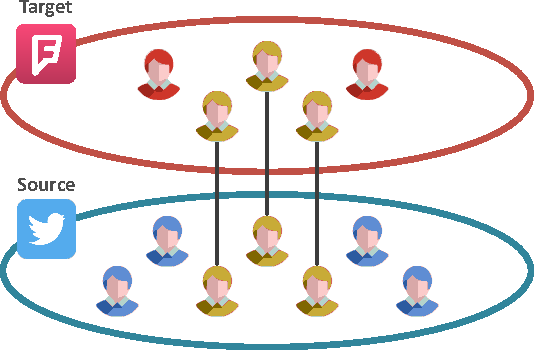
\includegraphics[width=2.5in]{snapshot-current.pdf}}
\hfil
\subfloat[Future snapshot]{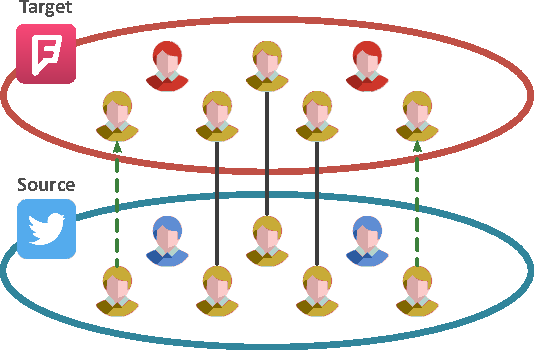
\includegraphics[width=2.5in]{snapshot-future.pdf}}
\caption{The formation of anchor links between source and target social networks. Blue and Red users are non-anchor users of the source and target networks, respectively. Users shown in yellow are anchor users and the links between them are anchor links. Intra-network links between users are omitted for better illustration. The figure on the left shows the current snapshot of both networks with three anchor users. The right figure shows the future snapshot in which another two non-anchor users from the source network have joined the target network and therefore two new anchor links (shown in dashed green arrows) have been formed.}
\label{fig:intro}
\end{figure*}

Predicting the formation of links in a social network have been studied extensively in recent years. However, the anchor link prediction problem studied in this paper is different from traditional link prediction tasks. The main difference comes from the fact that in conventional link prediction problems, both endpoints of the missing links are presented in the same network, while in anchor link prediction problem, one of the two endpoints (which is the target one) is missing and will be added to the target network once the anchor link is created. Moreover, the problem of "anchor link inference", which has proposed in \cite{kong2013}, is another related work that is totally different from anchor link prediction. In anchor link inference problem, the goal is to discover the correspondence between accounts of the same users across multiple networks. In other words, the goal of anchor link inference is to detect anchor links which exists in reality between networks, but are unknown. On the contrary, anchor link prediction problem aims to predict formation of anchor links in the future.


Preliminary works on link prediction had only concentrated on the network structure to predict the future links, while there are many other types of information, such as locations and posts contents, that can be leveraged. In order to use the abundant information in social networks, the recent trends in link prediction have changed their focus from homogeneous networks to heterogeneous ones \cite{davis2011, sun2011co, cao2014collective, zhang2013predicting}. Unlike homogeneous networks which are only composed of single type of nodes and links, in heterogeneous networks, multiple types of nodes are related using multiple types of links. For example, alongside with users and locations that can be considered as different node types of a heterogeneous social network, social links among users, and location links between users and locations, are instances of different kinds of links. In this paper, we have focused on prediction of anchor links by leveraging heterogeneous information, and formulated both the source and target networks as two heterogeneous social networks.

The anchor link prediction problem in heterogeneous networks is a challenging issue, and some of these challenges are as follows:

\begin{itemize}
\item \textit{Lack of features}:
The extraction of heterogeneous features that are capable of utilizing heterogeneous information of both source and target networks for the anchor link prediction problem is a challenging prerequisite which has not been addressed yet.

\item \textit{Missing target node}:
The conventional link prediction approaches cannot be extended to solve the anchor link prediction problem, since the target node is missing in the later one. This issue puts forward a big challenge to be addressed.

\item \textit{Network difference problem}:
The source and target networks may have different structure and characteristics. This problem which is referred to as heterogeneity between source and target networks in \cite{wu2014learning}, is another challenge of anchor link prediction.
\end{itemize}

In this paper, we propose a meta-path-based approach called CRMP (Connector and Recursive Meta-Paths) to solve the anchor link prediction problem. We use meta-paths as a powerful tool to model the effective social factors that affect a source user to join the target network. Using network schema of both the source and target networks, and existing anchor links, we introduce two meta-path categories: connector meta-paths and recursive meta-paths. Each of these two class of meta-paths model different aspects of social factors between anchor and non-anchor users and provide a feature building mechanism that are independent of the underlying networks. We formulate the problem as a binary classification task and utilize connector and recursive meta-paths to extract a feature vector for each non-anchor user to predict formation of anchor links. Extensive experiments on real-world social networks show that the proposed CRMP method outperforms the recent relevant methods.

The rest of this paper is organized as follows. Section \ref{sec:related} provides the related works. In section \ref{sec:problem}, we present the problem formulation. We will explain the proposed method in section \ref{sec:method}. Experiment results are discussed in section \ref{sec:experiments}. Finally, we conclude the paper in section \ref{sec:conclusion}.



\section{Related Works}\label{sec:related}

\begin{table*}[!t]
\renewcommand{\arraystretch}{1.3}
\caption{Summary of Related Works}\label{table:literature}
\centering
\begin{tabular}{|l||c|c|c|c|}
\hline
Property & Link Prediction \cite{liben2007link, lu2011link, al2011survey, wang2014review} & Anchor Link Inference \cite{kong2013, zhang2015integrated} & Anchor Link Prediction \cite{wu2014learning}\\
\hline\hline
Information Sources & Single/Multiple Networks & Multiple Networks & Multiple Networks\\
Network Type & Homogeneous/Heterogeneous & Heterogeneous & Homogeneous/Heterogeneous\\
Type of Links & Intra-Network Links & Missing Anchor Links & Future Anchor Links\\
Method & Supervised/Unsupervised & Supervised/Semi-Supervised & Unsupervised\\
\hline
\end{tabular}
\end{table*}

The problem of link prediction in social networks have been studied extensively in recent years \cite{liben2007link, lu2011link, al2011survey, wang2014review}, and many distinct methods have been proposed to solve this problem. Proximity-based approaches are from the earliest methods in which a measure of similarity like common neighbors, Jaccard coefficient, and Adamic/Adar index \cite{adamic2003friends} are defined between two nodes, and missing links are being ranked based on the this measure. Another class of methods are probabilistic methods \cite{clauset2008hierarchical, airoldi2009mixed, taskar2003link} in which a probabilistic model of link creation is fitted to the network data, and prediction is performed based on the probabilities inferred from the model.
In supervised classification-based methods \cite{al2006link}, a binary classifier is trained by using the feature vectors extracted for each link in the network, to predict links.

The preliminary works have been focused on homogeneous networks containing single type of nodes and links. Recently, the use of heterogeneous information in link prediction problem has gained much attention. Sun et al. \cite{sun2011co} used a meta-path-based approach called PathPredict to predict co-authorship links in heterogeneous bibliographic networks. Yang et al. \cite{yang2012link} proposed a probabilistic method called MRIP to predict links in heterogeneous networks. Cao et al. \cite{cao2014collective} also suggested a meta-path-based method to predict multiple type of links in heterogeneous information networks. Kuo et al. \cite{kuo2013unsupervised} devised an unsupervised method using aggregative statistics for link prediction problem in heterogeneous networks.

More recent works on link prediction were focused on using multiple heterogeneous social networks to enhance performance of link prediction tasks \cite{zhang2013predicting, zhang2014transferring, zhang2014meta}. Besides, the problem of anchor link inference were suggested by Kong et al. \cite{kong2013} and a method called MNA were proposed to detect unknown anchor links across multiple heterogeneous social networks. Zhang and Yu \cite{zhang2015integrated} also proposed a method called CLF to infer both anchor and social links, simultaneously.

Meanwhile, the problem of anchor link prediction has not gained much attention in the research community, until recently. To the best of our knowledge, the closest proposed method to the anchor link prediction problem, is the CICF method of Wu et al. \cite{wu2014learning}. The main idea of CICF is to transfer knowledge only through those anchor users who behave consistently across both the source and target networks. However, they formulated the problem as a cross-domain learning task, and thus missed some other important factors such as peer influence that affects the formation of anchor links. Furthermore, they did not intend to use heterogeneous information and the task of feature extraction is delegated to the application. 

Table \ref{table:literature} shows a comparison between link prediction, anchor link inference, and anchor link prediction problems.
Besides the conventional link prediction studies, there are other works that are related to the problem of anchor link prediction. In \cite{xu2014retaining}, the most important factors that cause users to switch between social networks are investigated, empirically. They used the Push-Pull-Mooring model of migration \cite{jackson1986aspects} as a basis, and categorized different factors into push, pull, and mooring. However, they did not propose a model for prediction of user migration in social networks. In another related work \cite{backstrom2006group}, Backstrom et al. have studied the formation and evolution of communities in social networks. They have shown that for a user, both number of her friends and the associated share of her friends' activities in the target community have great impact on her to join that community. We have used the results of these studies as a background theory for the proposed method.



\section{Problem Formulation}\label{sec:problem}
In this section, we will give the formal definitions of important concepts that have been used in this paper and the formulation of the anchor link prediction problem.

\subsection{Terminology Definition}
\begin{definition}{(Heterogeneous Social Network)}
A social network with multiple kinds of nodes and links is called a heterogeneous social network. It is represented as $G=(V,E)$ where $V=\bigcup_iV_i$ is the set of different nodes and $E=\bigcup_jE_j$ is the set of different links.
\end{definition}

\begin{definition}{(Network Schema \cite{sun2012mining})}
The schema of a heterogeneous network $G$ is a graph $S_G=(\nu, \varepsilon)$ where $\nu$ is the set of different node types and $\varepsilon$ is the set of different link types in $G$.
\end{definition}

\figurename~\ref{fig:schema} represents the schema of a heterogeneous social network, where \textit{user}, \textit{post}, \textit{location}, \textit{word}, and \textit{time} are considered as different node types, and \textit{follow}, \textit{write}, \textit{written at}, \textit{checkin at}, and \textit{contain} are different link types. 
In this paper, we have used Twitter and Foursquare (which are both heterogeneous social networks) as the source and target networks, respectively. They have the same schema as shown in \figurename~\ref{fig:schema}. However, the proposed framework does not depend on this specific network schema and one can define his own schemas for the source and target networks depending on the social networks used in application. Using this network schema, we formulate source and target networks as $G^g=(V^g,E^g)$ where $V^g=U^g\cup P^g\cup L^g\cup T^g\cup W^g$ in which $U^g$, $P^g$, $L^g$, $T^g$, and $W^g$ denotes the set of users, posts, locations, timestamps, and words relative to network $g=s$ or $t$, respectively. Moreover, we indicate node types with capital letters (like $U$ for user type) and node instances with small letters (like $u$ for a user instance).

\begin{figure}[!t]
\centering
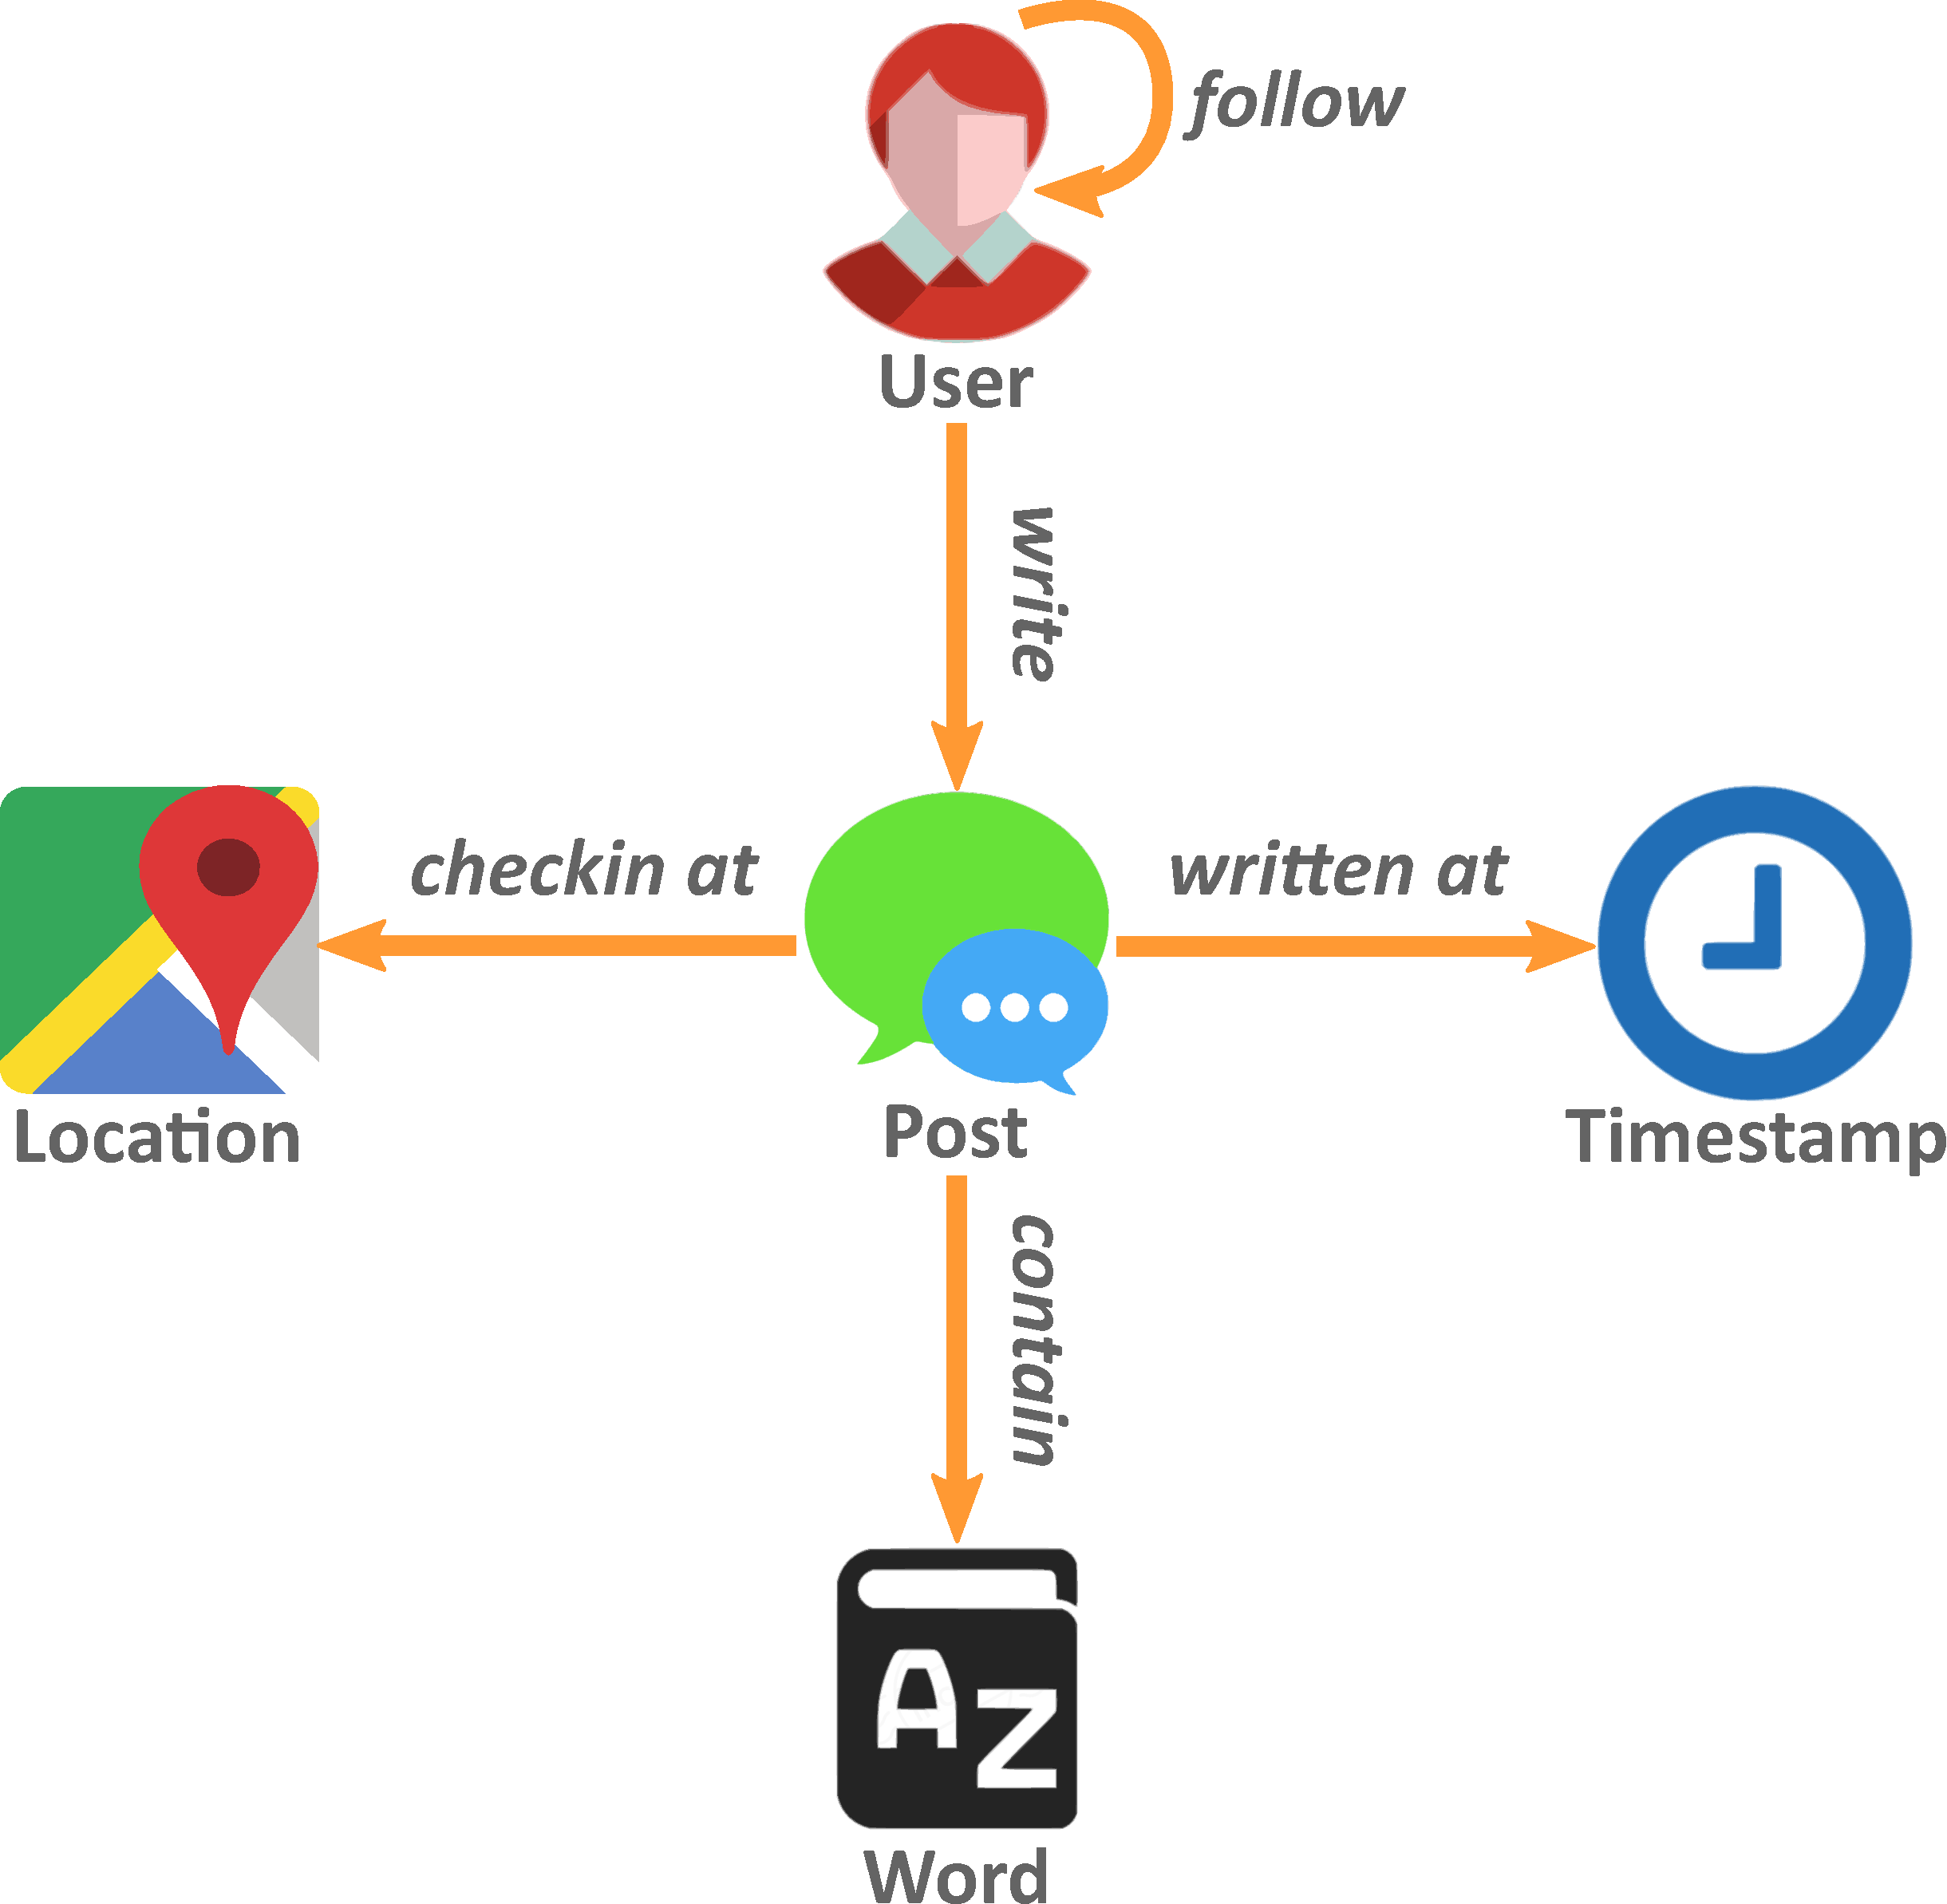
\includegraphics[width=2.5in]{schema.pdf}
\caption{Schema of a general heterogeneous social network}
\label{fig:schema}
\end{figure} 

\begin{definition}{(Meta-Path \cite{sun2012mining})}
A meta-path is any directed path along the network schema. Formally speaking, given a network schema $S_G=(\nu, \varepsilon)$, the sequence $\nu_1\xrightarrow{\varepsilon_1}\nu_2\xrightarrow{\varepsilon_2}\dots\nu_{k-1}\xrightarrow{\varepsilon_{k-1}}\nu_k$ is a meta-path defined on $S_G$ where $\nu_i\in \nu$ and $\varepsilon_i\in \varepsilon$. A meta-path is called homogeneous if all $\nu_i$s and all $\varepsilon_i$s be the same; otherwise it is called to be a heterogeneous meta-path.
\end{definition}

\begin{definition}{(Anchor Link)}
Given the source and target networks as $G^s$ and $G^t$, and their user sets as $U^s$ and $U^t$, the link $(u_i^s, u_j^t)$ is an anchor link between $G^s$ and $G^t$ if $u_i^s\in U^s$ and $u_j^t\in U^t$ and both $u_i^s$ and $u_j^t$ belong to the same user.
\end{definition}

Despite most prior works \cite{kong2013, zhang2013predicting, zhang2014transferring, zhang2014meta, zhang2015integrated} in which anchor links are considered to be undirected, we consider them as directed links. It is important to note that the direction of anchor links only indicates the network that the user joined recently.

\begin{definition}{(Joint Network Schema)}
Given the source and target networks as $G^s$ and $G^t$, and their network schemas $S_{G^s}$ and $S_{G^t}$, we create a new schema called \textit{joint network schema} as $S_{G^{(s,t)}}=(\nu^s\cup\nu^t, \varepsilon^s\cup\varepsilon^t\cup\{anchor\})$. That means we add anchor link as a new link type to the union of the source and target network schemas.
\end{definition}

\begin{definition}{(Anchor Meta-Path)}
Given the joint network schema, we define $\alpha(U^s,U^t)=U^s\xleftrightarrow{anchor}U^t$. Unlike anchor links, we consider anchor meta-paths as undirected, which means $\alpha(U^s,U^t)=\alpha(U^t,U^s)$
\end{definition}

\subsection{Anchor Link Prediction Problem}
We now formally define the anchor link prediction problem. Given two heterogeneous social networks $G^s$ and $G^t$ as the source and target networks, besides their network schemas $S_{G^s}$ and $S_{G^t}$ respectively, the goal of anchor link prediction is to predict the formation of anchor links $(u_i^s, u_j^t)$ where the user $u_j^t$ who is called target user, is not currently in the target network and will be joined in the future.

The key challenge of anchor link prediction is the fact that the target user is missing, and the formation of anchor link with the creation of target user have to be done simultaneously. Hence, conventional link prediction approaches cannot be applied to solve the anchor link prediction problem. In the next section, we propose the CRMP method which is a supervised approach to predict anchor links directed from the source to the target network.

\section{Proposed Method}\label{sec:method}

In this section, we introduce the proposed method called \textit{Connector and Recursive Meta-Paths} to solve the anchor link prediction problem in heterogeneous social networks. We first review the required background theories that our model is built upon them. Based on these theories, we then introduce connector meta-paths and recursive meta-paths which can effectively model the theories behind the joining a source users to the target network. Using these meta-paths, a feature vector is extracted for each non-anchor user from the source network that can be used to train a binary classifier to predict formation of new anchor links.

\subsection{Background}\label{sec:method:factors}

There are many factors that causes a non-anchor user from the source network to join the target network and so become an anchor one. As shown in \figurename~\ref{fig:factors}, we categorize these factors in two classes: personal and social factors.

\begin{figure}
\centering
%\colorlet{mygreen}{green!75!black}
%\colorlet{col1in}{red!10}
%\colorlet{col1out}{red!20}
%\colorlet{col2in}{mygreen!20}
%\colorlet{col2out}{mygreen!30}
%\colorlet{col3in}{yellow!20}
%\colorlet{col3out}{yellow!30}
%\colorlet{col4in}{mygreen!10}
%\colorlet{col4out}{mygreen!20}
%\colorlet{col5in}{yellow!10}
%\colorlet{col5out}{yellow!20}
%\colorlet{linecol}{blue!60}
%
%\pgfkeys{/forest,  
%  ellip/.append style  = {ellipse, inner color = col5in,
%                          outer color = col5out},
%}
%\begin{forest}
%  for tree={
%      font=\tiny,
%      line width=1pt,
%      draw=linecol,
%      ellip,
%      align=center,
%      child anchor=north,
%      parent anchor=south,
%      l sep+=12.5pt,
%      edge path={
%        \noexpand\path[color=linecol, rounded corners=5pt,
%          >={Stealth[length=10pt]}, line width=1pt, ->, \forestoption{edge}]
%          (!u.parent anchor) -- +(0,-5pt) -|
%          (.child anchor)\forestoption{edge label};
%        },
%      where level={3}{tier=tier3}{},
%      where level={0}{l sep-=15pt}{},
%      where level={1}{
%        if n={1}{
%          edge path={
%            \noexpand\path[color=linecol, rounded corners=5pt,
%              >={Stealth[length=10pt]}, line width=1pt, ->,
%              \forestoption{edge}]
%              (!u.west) -| (.child anchor)\forestoption{edge label};
%            },
%        }{
%          edge path={
%            \noexpand\path[color=linecol, rounded corners=5pt,
%              >={Stealth[length=10pt]}, line width=1pt, ->,
%              \forestoption{edge}]
%              (!u.east) -| (.child anchor)\forestoption{edge label};
%            },
%        }
%      }{},
%  }
%  [Important Factors, inner color=col1in, outer color=col1out
%    [Personal Factors, inner color=col2in, outer color=col2out
%      [Attractiveness\\of the target\\network, inner color=col4in, outer color=col4out]
%      [Dissatisfaction\\from the source\\network, inner color=col4in, outer color=col4out]
%    ]
%    [Social Factors, inner color=col3in, outer color=col3out
%      [Number of\\friends in the\\target network]
%      [Intimacy\\between friends in\\the target network]
%    ]
%  ]
%\end{forest}
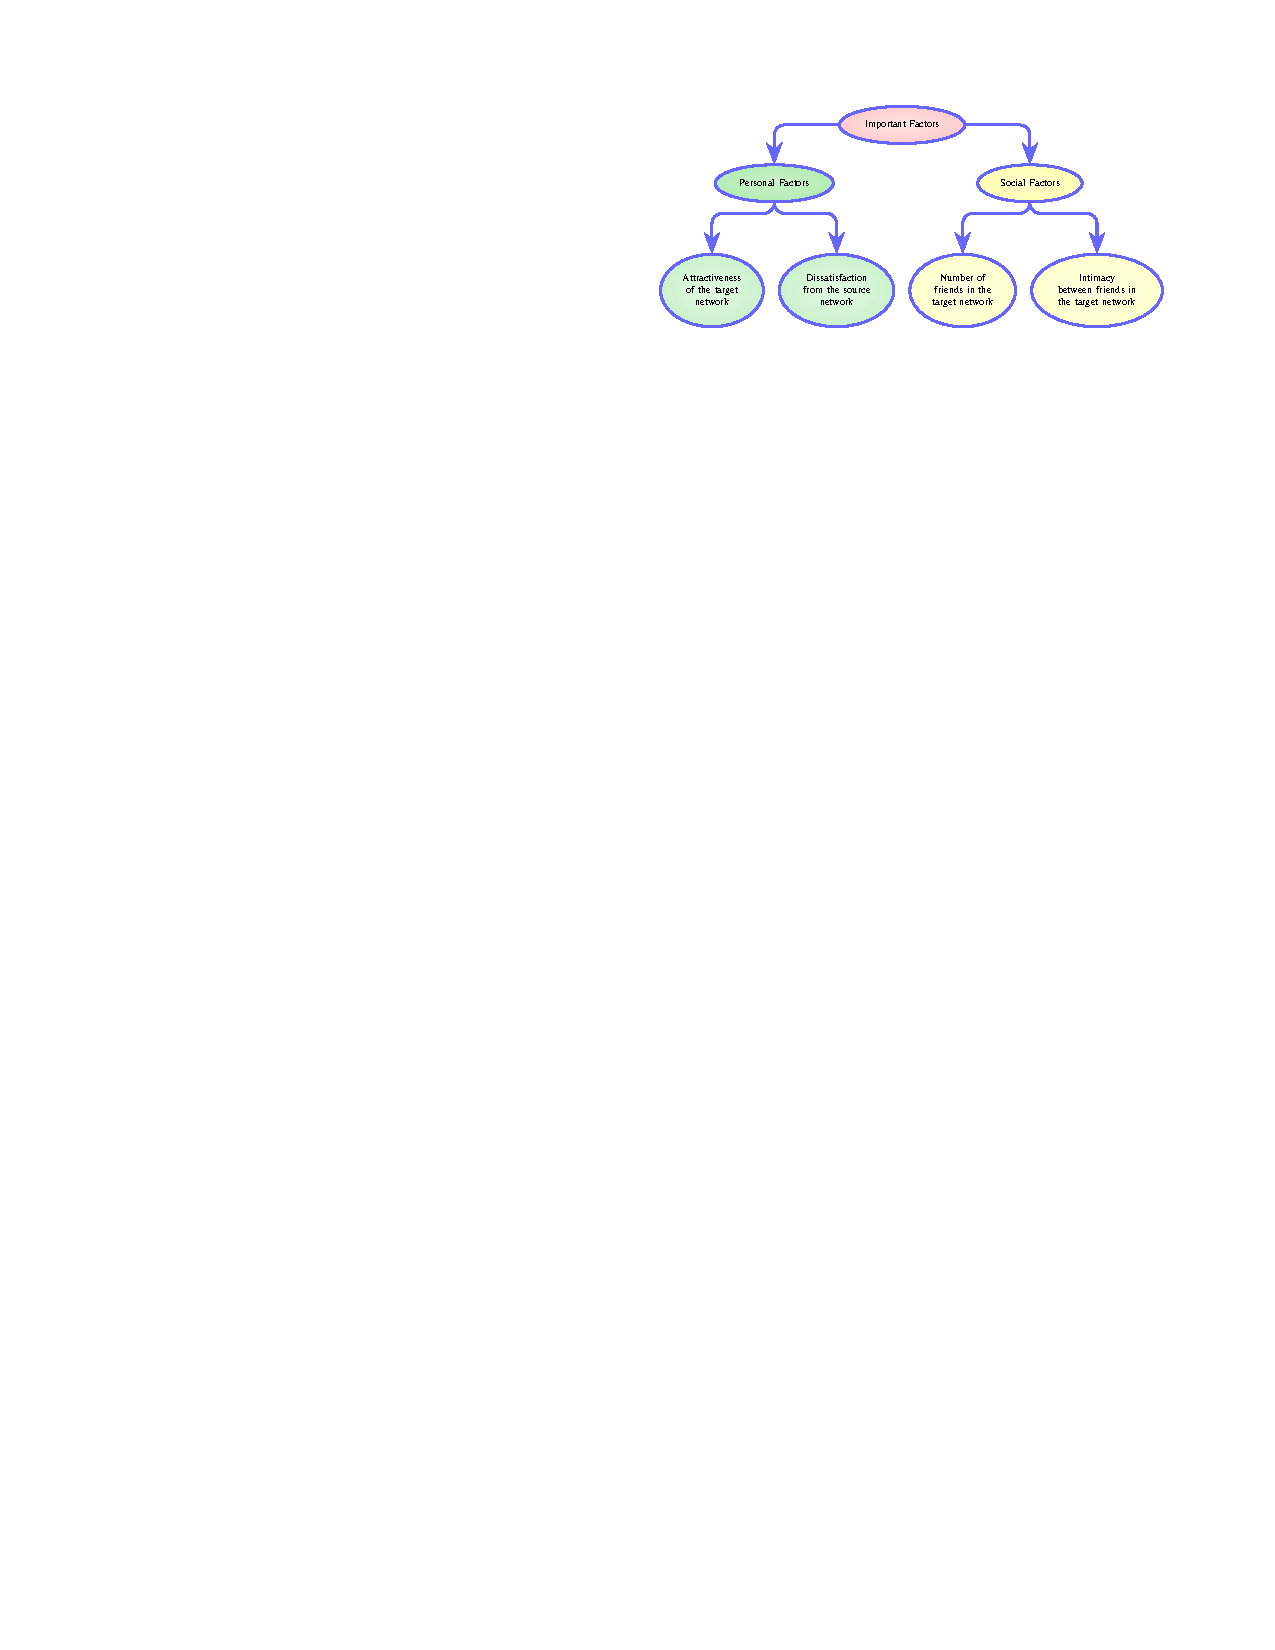
\includegraphics[scale=1]{factors.pdf}
\caption{Different factors affecting a source user to join the target network.}
\label{fig:factors}
\end{figure}

Personal factors are those factors that are related to the user profile itself. There are two main personal factors affecting a source user to join the target network. First, the dissatisfaction with the source network; and second, the attractiveness of the target network \cite{xu2014retaining}.
On the other hand, social factors which are called \textit{peer influence} in \cite{xu2014retaining}, are the influence of friends who have already joined the target network. We consider the effect of peer influence in two folds: first, the number of user's friends who are already joined the target network; and second, the amount of activity, similarity, and connections between those friends in the target network, which we call \textit{intimacy between friends}. The more number of a source user's friends and intimacy between them in the target network, the more likely she is to join the target network.

In this paper, we just use social factors because of two reasons. First, according to \cite{xu2014retaining}, peer influence is more effective than other factors in user intension to move from a social network to a new one. Second, the modeling of social factors can be generalized over different social networks, whereas personal factors are network dependent. In the following, we introduce connector and recursive meta-paths by which we model different social factors that results in formation of new anchor links.

\subsection{Connector Meta-Paths}\label{sec:method:connector}

As we mentioned, an important social factor that affects a source user to become a target one is the number of her friends in the target network. For a source user $u^s$, the number of her followees who are in the target network can be found by counting the instances of the following meta-path starting with $u^s$:
\begin{equation*}\label{eq:neighborcount}
U^s\xrightarrow{follow}U^s\xleftrightarrow{anchor}U^t
\end{equation*}

We now claim that not only the direct followees of a source user are effective in the user intension to join the target network, but also the user would be influenced by other anchor users who are in a way \textit{similar} to that user. The reason behind this, is that the similar users often fall in the same community, and the users of a community usually perform similar actions and take similar decisions. For example, if a user belong to a community of educated people, and most of them have join a new social network, it means that the new social network is appropriate for educated people. As a result, being similar to anchor users is positively correlated with a non-anchor user's intension to join the target network. Therefore, we extend the "follow" relation in aforementioned meta-path with a similarity relationship. We call the action of extending friendship relation with similarity relationship to be \textit{similarity extension}. In order to model similarity between users, we define the notion of \textit{similarity meta-paths}.

\begin{definition}{(Similarity Meta-Path)}
Given a network schema $S_G$, a meta-path $\sigma(U,U) = U\xrightarrow{R_1}\dots\xrightarrow{R_k}U$ denoted as $U\rightsquigarrow U$, is called a similarity meta-path on $S_G$ if it is able to capture the similarity between endpoint users.
\end{definition}


We do not impose any restrictions on choosing similarity meta-paths. Depending on the real application, one can define her own meta-paths based on the schema of the source and target networks in use. For the network schema shown in \figurename~\ref{fig:schema}, we suggest the following meta-paths proposed in \cite{zhang2014meta}:

\begin{itemize}
\item $\sigma_1(U,U)=U\xrightarrow{follow}U$
%\\denoted as $U\rightarrow U$
\item $\sigma_2(U,U)=U\xrightarrow{follow^{-1}}U$
%\\ denoted as $U\leftarrow U$
\item $\sigma_3(U,U)=U\xrightarrow{follow}U\xrightarrow{follow}U$
%\\ denoted as ${U\rightarrow U\rightarrow U}$
\item $\sigma_4(U,U)=U\xrightarrow{follow}U\xrightarrow{follow^{-1}}U$
%\\ denoted as ${U\rightarrow U\leftarrow U}$
\item $\sigma_5(U,U)=U\xrightarrow{follow^{-1}}U\xrightarrow{follow}U$
%\\ denoted as ${U\leftarrow U\rightarrow U}$
\item $\sigma_6(U,U)=U\xrightarrow{follow^{-1}}U\xrightarrow{follow^{-1}}U$
%\\ denoted as ${U\leftarrow U\leftarrow U}$
\item $\sigma_7(U,U)=U\xrightarrow{write}P\xrightarrow{checkin\ at}L\xrightarrow{checkin\ at^{-1}}P\xrightarrow{write^{-1}}U$
%\\ denoted as ${U\rightarrow P\rightarrow L\leftarrow P\leftarrow U}$
\item $\sigma_8(U,U)=U\xrightarrow{write}P\xrightarrow{written\ at}T\xrightarrow{written\ at^{-1}}P\xrightarrow{write^{-1}}U$
%\\ denoted as ${U\rightarrow P\rightarrow T\leftarrow P\leftarrow U}$
\item $\sigma_9(U,U)=U\xrightarrow{write}P\xrightarrow{contain}W\xrightarrow{contain^{-1}}P\xrightarrow{write^{-1}}U$
%\\ denoted as ${U\rightarrow P\rightarrow W\leftarrow P\leftarrow U}$
\end{itemize}

The meta-paths $\sigma_1$ to $\sigma_6$ are \textit{social similarity meta-paths} which only use social relations to capture similarity between two users. On the other hand, the meta-paths $\sigma_7$ to $\sigma_9$ which are called \textit{spatial}, \textit{temporal}, and \textit{textual similarity meta-paths}, can use heterogeneous informations such as locations, timestamps, and words to capture similarity of endpoint users, respectively.

With the definition of similarity meta-paths, we now define the notion of \textit{connector meta-paths}.

\begin{definition}{(Connector Meta-Path)}
A connector meta-path is defined as:
\begin{equation}
\Psi_i(U^s,U^t)=\sigma^s_i(U^s,U^s)\circ\alpha(U^s,U^t)
\end{equation}
where $\sigma\circ\alpha$ denotes the composition of relations $\sigma$ and $\alpha$.
\end{definition}

A connector meta-path \textit{connects} a source user to the target network using a similarity meta-path. It can be easily seen that the meta-path $U^s\xrightarrow{follow}U^s\xleftrightarrow{anchor}U^t$ which were used to count the number of followees of a source user $u^s$, who have joined the target network, is a special case of connector meta-path when we use $\sigma_1(U,U)$ as the similarity meta-path.

\subsection{Recursive Meta-Paths}

Another important social factor that affects a source user to become a member of the target network, as we talked about in section \ref{sec:method:factors}, is the level of intimacy between friends of that user in the target network. Thus, we need to model the intimacy between different users on the target network. To this end, we use the same similarity meta-paths introduced in section \ref{sec:method:connector} as a measure of intimacy between users of the target network. The intuition behind this, is that if two users be more similar to each other, and have done more common activities, then more instances of similarity meta-paths would exist between them. Based on this fact, for a non-anchor user from the source network, we model the intimacy between her friends in the target network by using the following meta-path:
\[
U^s\xrightarrow{follow}U^s\xleftrightarrow{anchor}U^t\rightsquigarrow U^t\xleftrightarrow{anchor}U^s\xrightarrow{follow^{-1}}U^s
\]

The instances of above meta-path which start and end with the same user $u^s$, means that $u^s$ has followed some users in the source network, who have already joined the target network and they are connected to each other via similarity meta-paths in the target network. Therefore, the existence of more instances of this meta-path means that a greater number of her friends are connected in the target network, and thus the likelihood of joining the user to the target network is higher. Similar to what we did in section \ref{sec:method:connector}, instead of using only direct followees of $u^s$, we extend this case using similarity extension as well which results in the definition of recursive meta-paths.

\begin{definition}{(Recursive Meta-Path)}
A recursive meta-path is defined as:
\begin{equation}
\Phi_{i,j,k}(U^s,U^s)=\Psi_i(U^s,U^t)\circ\sigma_j^t(U^t,U^t)\circ\Psi_k^{-1}(U^t,U^s)
\end{equation}
\end{definition}
 
We call this class of meta-paths "recursive" because their instances form cycles, which means for a source user $u^s$, the path begins with  $u^s$, goes to the target network and then comes back to the source network via anchor links, and finally returns to $u^s$ herself. Recursive meta-paths show that similar users to $u^s$ in the source network, are also similar to each other in the target network. As a result, existence of a great number of instances of this meta-paths means that the members of the communities in the source network, also form communities in the target network, which is positively correlated with the intension of $u^s$ to join the target network.

\subsection{Classification}
Based on the meta-paths we introduced in the previous sections, for each user in the source network, we can extract a feature vector that can be used in a supervised (or semi-supervised) classification method. The "path count" measure proposed in \cite{sun2012mining} can be used to extract features from meta-paths. More formally, let $f_{\Psi_i}$ be the feature value based on connector meta-path $\Psi_i$:
\begin{equation}
f_{\Psi_i}(u^s)=\sum_{u^t\in U^t}PC_{\Psi_i}(u^s,u^t)
\end{equation}
where $PC_{\Psi_i}$ denotes the path count of meta-path $\Psi_i$, which is the number of path instances between $u^s$ and $u^t$ following the meta-path $\Psi_i$. In this way, assuming there are $c$ different similarity meta-paths defined for the source network, the \textit{connector feature vector} for user $u^s$ would be of the form:
\begin{equation}
\Psi_F(u^s) = [f_{\Psi_1}(u^s), f_{\Psi_2}(u^s), \dots, f_{\Psi_c}(u^s)]^T
\end{equation}
Similarly, let $f_{\Phi_{i,j,k}}$ be the feature value based on recursive meta-path $\Phi_{i,j,k}$:
\begin{equation}
f_{\Phi_{i,j,k}}(u^s)=PC_{\Phi_{i,j,k}}(u^s,u^s)
\end{equation}
where $PC_{\Phi_{i,j,k}}$ denotes the path count of meta-path $\Phi_{i,j,k}$, then the \textit{recursive feature vector} for user $u^s$ would be as follows:
\begin{equation}
\Phi_F(u^s) = [f_{\Phi_{1,1,1}}(u^s), f_{\Phi_{1,1,2}}(u^s), \dots, f_{\Phi_{c,r,c}}(u^s)]^T
\end{equation}
assuming there are $c$ different similarity meta-paths defined for the source network and $r$ different similarity meta-paths defined for the target network.
The CRMP method utilizes both connector and recursive feature vectors in the form of $\left[\Psi_F^T(u^s),\Phi_F^T(u^s)\right]^T$ to train a classifier in order to predict formation of anchor links initiated by the source non-anchor users.

\section{Experiments}\label{sec:experiments}
We conducted extensive experiments to test the effectiveness of CRMP method by using real-world dataset. In this section, we first introduce the dataset and explain the experiment settings. Finally, we discuss about the experimental results.

\subsection{Datasets}
We used a heterogeneous dataset, composed of Twitter and Foursquare which have previously used in \cite{zhang2014meta, zhang2014transferring, zhang2013predicting, zhang2015integrated}. In addition to the structure of the two networks, we used locations, timestamps and text contents of the posts from both networks as heterogeneous information. During experiments, Twitter is used as the source network, and Foursquare (which is a newer network than Twitter) is used as the target network. The detailed statistics of these networks is presented in Table \ref{table:dataset}.

\begin{table}
\centering
\caption{Properties of Source and Target Networks}
\label{table:dataset}
\begin{tabular}{l l c c}
\toprule
& & \multicolumn{2}{c}{Network} \\
\cmidrule(l){3-4}
& Property & \textbf{Twitter} (Source) & \textbf{Foursquare} (Target)\\
\midrule % In-table horizontal line
& User & 5,223 & 3,456 \\ % Content row 1
\# Node & Tweet/Tip & 8,205,030 & 48,585 \\ % Content row 2
& Location & 257,253 & 38,861 \\ % Content row 3
\midrule
& Follow & 164,919 & 16,890 \\ % Content row 1
\# Link & Write & 8,205,030 & 48,585 \\ % Content row 2
& Check-in & 516,149 & 48,585 \\ % Content row 3
\bottomrule % Bottom horizontal line
\end{tabular}
\end{table}

For each user of Twitter network, we used Twitter API to obtain the date she joined the network. Since the Foursquare API does not provide such capability, for each Foursquare user, we used the date of her first tip as the creation date of that user. A total of 3282 anchor users exist where about 1900 of them who have joined the target network after joining the source network, were used as ground truth to evaluate the performance of different methods including the proposed CRMP. The remaining anchor users were kept as existing anchor links between two networks.

\subsection{Experiment Settings}

\subsubsection{Comparison Methods}
In order to evaluate the performance of CRMP, we used the following methods:
\begin{itemize}
\item \textbf{CICF}: This method proposed in \cite{wu2014learning} is the only method presented so far for the problem of anchor link prediction.
\item \textbf{CMP}: This method is a variant of CRMP, which utilizes connector meta-paths only. This method is particularly used to analyze the effect of connector meta-paths in prediction of anchor links.
\item \textbf{RMP}: This method is a variant of CRMP, which utilizes recursive meta-paths only. This method is particularly used to analyze the effect of recursive meta-paths in prediction of anchor links.
\end{itemize}

\subsubsection{Performance Measures}
We evaluated the prediction performance of different methods under different setting using Accuracy and AUC measures. Because CICF can only output scores, for calculating Accuracy, we ranked the users according to their scores and selected top-k users as positively classified, and the remaining as negatively classified, where k is chosen equivalent to the number of positive samples.

\subsubsection{Experiment Setups}
Anchor users who have joined the source network before the target network are selected as positive users set, whose number is 1936, and non-anchor users formed the negative users set, whose number is 1941. The target node of positive users were removed from the target network. For CICF method, the optimal parameters were found by using the grid search, and path count of similarity meta-paths were used as feature vector for edges. For CRMP and its variants, Support Vector Machines (SVM) with linear kernel and default parameters were used as the base classifier. We used 5-fold cross-validation for performance evaluation: 4 folds are used for training set and remaining 1-fold is used as the test set.

\subsection{Experiment Results}
We first evaluated the prediction performance of all methods, using both homogeneous features (which are extracted using social similarity meta-paths only) and heterogeneous ones (which are extracted using social, spatial, temporal, and textual similarity meta-paths), to see the effect of different feature sets on different methods in anchor link prediction. Since the number of existing anchor links between two networks is an important factor that affects the performance of anchor link prediction, we then compared the impact of different number of existing anchor links on all methods. Next, regarding the fact that the application of anchor link prediction is for new target networks, we analyzed the effect of different degrees of newness for the target network on different methods. Finally, we evaluated the effectiveness of similarity extension to verify our assertion about extending "follow" relation with similarity relationship in both connector and recursive meta-paths.

\subsubsection{Effect of heterogeneous information}
In \figurename~\ref{fig:het}, we compared the performance of all methods using homogeneous and heterogeneous features to test the effectiveness of those features. The figure depicts that CRMP outperforms other methods under both Accuracy and AUC, using either homogeneous or heterogeneous features. Heterogeneous features increased the Accuracy of CMP, RMP, CRMP and CICF methods by about 2.5\%, 8.5\%, 3\% and 7\%, respectively. Under AUC, heterogeneous features result in an improvement of 1\% on CMP, 4\% on RMP, 3\% on CRMP, and 2.5\% on CICF. According to the results shown in the figure, using heterogeneous features, CRMP performs over 40\% better than CICF under Accuracy, and over 60\% under AUC. It can be induced that, RMP performs better than CMP, yet not better than CRMP. As a result, using connector and recursive meta-paths together is the most effective approach in anchor link prediction, while using connector meta-paths exclusively, is the least.

\newcommand{\hetplot}[1]{
\begin{tikzpicture}
\begin{axis}
[
ybar,
tiny,
width=1.9in,
enlarge x limits=0.4,
bar width=0.07in,
legend style={at={(0.5,1.3)},
anchor=north,legend columns=-1, draw=none},
symbolic x coords={CMP, RMP, CRMP, CICF},
xtick=data,
ymin=0.4,
ymajorgrids,
y tick label style={
/pgf/number format/.cd,
fixed,
fixed zerofill,
precision=2,
/tikz/.cd
},
]
\addplot+[
fill=orange,
draw=red,
error bars/.cd,y dir=both,y explicit,error mark=.] table[x=Method,y=Value, y error=Error] {results/het-#1-sc.dat};
\addplot+[
fill=cyan,
draw=blue,
error bars/.cd,y dir=both,y explicit,error mark=.] table[x=Method,y=Value, y error=Error] {results/het-#1-sc-sp-tp-tx.dat};
\legend{Homogeneous, Heterogeneous}
\end{axis}
\end{tikzpicture}
}

\begin{figure}[!t]
\centering
\subfloat[Accuracy]{
\hetplot{acc}
\label{fig:het:acc}}
\hfil
\subfloat[AUC]{
\hetplot{auc}
\label{fig:het:auc}}
\caption{Comparison of different methods using homogeneous and heterogeneous features with $\gamma_A=0.8$ and $\gamma_T=1$.}
\label{fig:het}
\end{figure}

\subsubsection{Effect of remaining anchor links}
We kept a fraction of randomly sampled existing anchor links under the control of parameter $\gamma_A$ which changes within $\{0.1,0.2,\dots,0.8\}$ and removed the remaining anchor links. The results are represented in \figurename~\ref{fig:ra}. As shown in the figure, it can be seen that CRMP method outperforms all other baselines consistently under both Accuracy and AUC measures. Under Accuracy and on average, CRMP is about 36.5\% better than CICF, 2.5\% better than RMP and 5.5\% better than CMP. Under AUC, CRMP is about 54\% better than CICF, 1\% better than RMP and 5\% better than CMP. We can see from the figure that as $\gamma_A$ gradually increases, the results of RMP and CRMP tend to become better, but CMP does not. This happens because as the number of anchor links increase, RMP and CRMP can leverage more information from the target network, but CMP, which does not utilize any information from the target network, remains approximately constant.

\newcommand{\anchorplot}[2]{
\begin{tikzpicture}
\begin{axis}
[
tiny,
width=1.9in,
legend style={at={(0.5,1.31)},
/tikz/every even column/.append style={column sep=0.2cm},
      anchor=north,legend columns=2, draw=none},
legend cell align=center,
ymin=0.45,ymax=#2,
xmin=0.0,xmax=0.9,
xtick={0.1, 0.2, 0.3, 0.4, 0.5, 0.6, 0.7, 0.8},
xmajorgrids,
ymajorgrids,
y tick label style={
    /pgf/number format/.cd,
        fixed,
        fixed zerofill,
        precision=2,
    /tikz/.cd
},
legend entries={CICF, CRMP, RMP, CMP},
]
\addplot[color=darkgray,thick,error bars/.cd,y dir=both,y explicit,] table[y error=e] {results/anchor-#1-cicf-ht.dat};
\addplot[color=cyan,thick,error bars/.cd,y dir=both,y explicit,] table[y error=e] {results/anchor-#1-crmp-ht.dat};
\addplot[color=orange,thick,error bars/.cd,y dir=both,y  explicit,] table[y error=e] {results/anchor-#1-rmp-ht.dat};
\addplot[color=purple,thick,error bars/.cd,y dir=both,y  explicit,] table[y error=e] {results/anchor-#1-cmp-ht.dat};
\end{axis}
\end{tikzpicture}
}

\begin{figure}[!t]
\centering
\subfloat[Accuracy]{
\anchorplot{acc}{0.75}
\label{fig:ra:acc}
}
%\hfil
\subfloat[AUC]{
\anchorplot{auc}{0.8}
\label{fig:ra:auc}}
\caption{Effect of remaining anchor link ratio $\gamma_A$ on performance of different methods. $\gamma_T$ is set to 1.}
\label{fig:ra}
\end{figure}

\subsubsection{Effect of newness of target network}
To represent different degrees of newness for the target network, we randomly sampled a fraction of information, including social links and tips, from the target network as available information under the control of parameter $\gamma_T$, and removed remaining information. We set $\gamma_A$ to 0.8 and changed $\gamma_T$ within $\{0.1,0.2,\dots,0.8\}$. The results are shown in \figurename~\ref{fig:rf} under the evaluation of Accuracy and AUC. Results of CMP is omitted because CMP does not utilize any information from the target network. The results show that CRMP method performs consistently better than all other methods under different degrees of newness of the target network. On average, the Accuracy achieved by CRMP is about 36\% better than CICF and 2.5\% better than RMP. Under AUC, CRMP performs about 56.5\% better than CICF and 1.5\% better than RMP. We can also see that the performance of RMP and CRMP slightly goes down while $\gamma_T$ decreases. This result shows that when the target network is new and sparse, the CRMP method can still achieve good performance.

\newcommand{\targetplot}[2]{
\begin{tikzpicture}
\begin{axis}
[
tiny,
width=1.9in,
legend style={at={(0.5,1.31)},
/tikz/every even column/.append style={column sep=0.2cm},
      anchor=north,legend columns=2, draw=none},
legend cell align=center,
ymin=0.45,ymax=#2,
xmin=0.0,xmax=0.9,
xtick={0.1, 0.2, 0.3, 0.4, 0.5, 0.6, 0.7, 0.8},
xmajorgrids,
ymajorgrids,
y tick label style={
    /pgf/number format/.cd,
        fixed,
        fixed zerofill,
        precision=2,
    /tikz/.cd
},
legend entries={CICF, CRMP, RMP},
]
\addplot[color=darkgray,thick,error bars/.cd,y dir=both,y explicit,] table[y error=e] {results/target-#1-cicf-ht.dat};
\addplot[color=cyan,thick,error bars/.cd,y dir=both,y explicit,] table[y error=e] {results/target-#1-crmp-ht.dat};
\addplot[color=orange,thick,error bars/.cd,y dir=both,y explicit,] table[y error=e] {results/target-#1-rmp-ht.dat};
\end{axis}
\end{tikzpicture}
}

\begin{figure}[!t]
\centering
\subfloat[Accuracy]{
\targetplot{acc}{0.75}
\label{fig:rf:acc}}
\hfil
\subfloat[AUC]{
\targetplot{auc}{0.8}
\label{fig:rf:auc}}
\caption{Effect of remaining information ratio $\gamma_T$ of the target network on performance of different methods. $\gamma_A$ is set to 0.8.}
\label{fig:rf}
\end{figure}

\newcommand{\hpiplot}[1]{
\begin{tikzpicture}
\begin{axis}
[
ybar,
tiny,
width=1.9in,
enlarge x limits=0.4,
bar width=0.07in,
legend style={at={(0.5,1.3)},
anchor=north,legend columns=-1, draw=none},
symbolic x coords={CMP, RMP, CRMP},
xtick=data,
ymin=0.5,ymax=0.8,
ymajorgrids,
y tick label style={
/pgf/number format/.cd,
fixed,
fixed zerofill,
precision=2,
/tikz/.cd
},
]
\addplot+[
error bars/.cd,
y dir=both,
y explicit,error mark=.] table[x=Method,y=Value, y error=Error] {results/hpi-np-#1.dat};
\addplot+[
error bars/.cd,
y dir=both,
y explicit,error mark=.] table[x=Method,y=Value, y error=Error] {results/hpi-wp-#1.dat};
\legend{No-SE, With-SE}
\end{axis}
\end{tikzpicture}
}

\begin{figure}[!t]
\centering
\subfloat[Accuracy]{
\hpiplot{acc}
\label{fig:hpi:acc}}
\hfil
\subfloat[AUC]{
\hpiplot{auc}
\label{fig:hpi:auc}}
\caption{Effect of similarity extension on performance of different methods with $\gamma_A=0.8$ and $\gamma_T=1$.}
\label{fig:hpi}
\end{figure}

\subsubsection{Effect of similarity extension}
We evaluated the correctness of similarity extension (SE) on CMP, RMP, and CRMP methods. By using only $\sigma_1^s$ in building connector and recursive meta-paths, we can ignore the effect of similarity extension on these methods. \figurename~\ref{fig:hpi} shows the Accuracy and AUC of No-SE and With-SE versions of CRMP and its variants. The results clearly demonstrate that applying similarity extension improved the performance of all methods considerably. Under Accuracy, similarity extension results in about 9\% improvement in CMP, 20\% improvement in RMP, and 16\% improvement in CRMP. Under AUC, similarity extension increased the result of CMP by about 14\%, RMP by about 22\% and CRMP by about 22\%. 

\section{Conclusion}\label{sec:conclusion}
In this paper, we studied the problem of anchor link prediction between heterogeneous social networks, and proposed an effective method called CRMP to solve the problem. To model the social factors affecting source users to become target ones, two class of meta-paths, \textit{connector} and \textit{recursive} meta-paths, were proposed which are built from smaller \textit{similarity} meta-paths that capture the similarity between users. By using these meta-paths, a feature vector was extracted for each non-anchor user and used in a supervised classification to predict the formation of anchor links. Extensive experiments performed on real-world dataset of Twitter and Foursquare demonstrate that CRMP outperforms the recent relevant methods.

There are many possible future directions for this work. Performing dimensionality reduction to reduce the number of features, beside using semi-supervised methods such as PU link prediction \cite{zhang2014meta}, can result in lower complexity and better prediction performance. Even though waiving personal factors brought simplicity to our model, it can be considered as a shortcoming for our approach. Thus, a potential study is to model personal factors and any other reasonable factors. Another interesting issue is to model the anchor link prediction using a temporal model to predict not only the formation of anchor links, but also the time of the formation of these links.


\section*{Acknowledgment}
We would like to thank Jiawei Zhang and Hao-Heng Chien for providing the Twitter and Foursquare dataset, and the source code of CICF, respectively. We also appreciate Reza Hadi Mogavi and Sina Jafarzadeh for their valuable comments, and ICT Innovation Center of Sharif University of Technology for its financial support.

% trigger a \newpage just before the given reference
% number - used to balance the columns on the last page
% adjust value as needed - may need to be readjusted if
% the document is modified later
\IEEEtriggeratref{5}
% The "triggered" command can be changed if desired:
%\IEEEtriggercmd{\enlargethispage{-5in}}

% references section

% can use a bibliography generated by BibTeX as a .bbl file
% BibTeX documentation can be easily obtained at:
% http://mirror.ctan.org/biblio/bibtex/contrib/doc/
% The IEEEtran BibTeX style support page is at:
% http://www.michaelshell.org/tex/ieeetran/bibtex/
\bibliographystyle{IEEEtran}
% argument is your BibTeX string definitions and bibliography database(s)
\bibliography{IEEEabrv,references}
%
% <OR> manually copy in the resultant .bbl file
% set second argument of \begin to the number of references
% (used to reserve space for the reference number labels box)
% \begin{thebibliography}{1}

% \bibitem{IEEEhowto:kopka}
% H.~Kopka and P.~W. Daly, \emph{A Guide to \LaTeX}, 3rd~ed.\hskip 1em plus
%   0.5em minus 0.4em\relax Harlow, England: Addison-Wesley, 1999.

% \end{thebibliography}




% that's all folks
\end{document}


